
%(BEGIN_QUESTION)
% Copyright 2012, Tony R. Kuphaldt, released under the Creative Commons Attribution License (v 1.0)
% This means you may do almost anything with this work of mine, so long as you give me proper credit

Use the ``impedance triangle'' to calculate the magnitude ($Z$) and phase angle ($\theta$) of total impedance within this series circuit containing resistance ($R$) and inductive reactance ($X$):

$$\includegraphics[width=15.5cm]{i01936x01.eps}$$

\vskip 20pt

$Z$ =

\vskip 10pt

$\theta$ = 

\underbar{file i01936}
%(END_QUESTION)





%(BEGIN_ANSWER)

$Z$ = 625 $\Omega$

\vskip 10pt

$\theta$ = 36.87$^{o}$

%(END_ANSWER)





%(BEGIN_NOTES)

{\bf This question is intended for exams only and not worksheets!}.

%(END_NOTES)


